\documentclass[../document.tex]{subfiles}
\begin{document}\label{ssec:time}
	
The Cyclic Redundancy Check {\tt crc} benchmark represents the Combinational Logic dwarf.
Figure~\ref{fig:time-crc} shows the execution times for the {\tt crc} benchmark over 50 iterations on each of the target architectures, including the KNL.
This is the only benchmark which performs best on CPU-type architectures, and it also performs well on the KNL MIC architecture.
All other benchmarks perform best on GPU type accelerators; furthermore, the performance on the KNL is poor due to the lack of support for wide vector registers in Intel's OpenCL SDK.
For the remaining benchmarks, we omit results for KNL.

\begin{figure}[h]
	\centering
	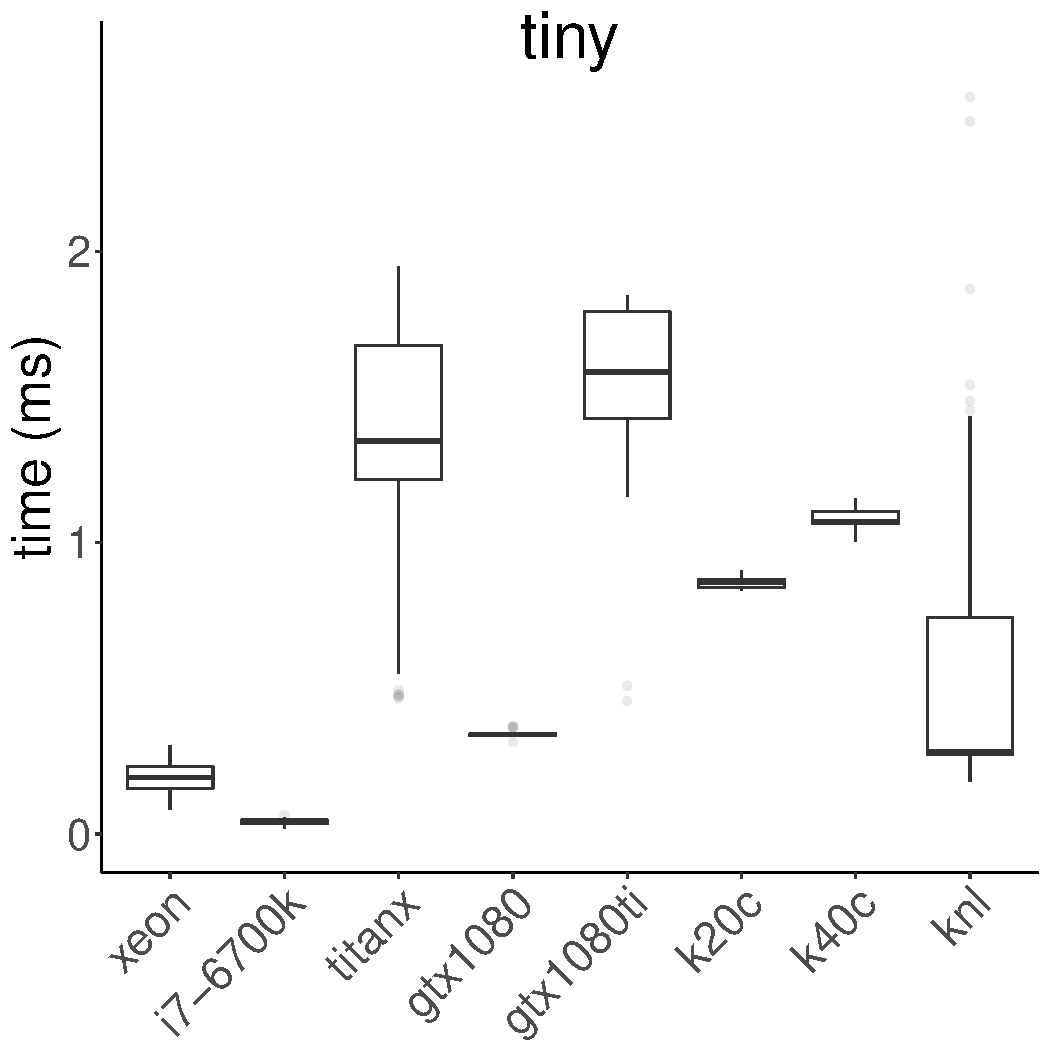
\includegraphics[width=0.23\textwidth]{figures/time-results/generate_crc_tiny_boxplot_knl-1}
	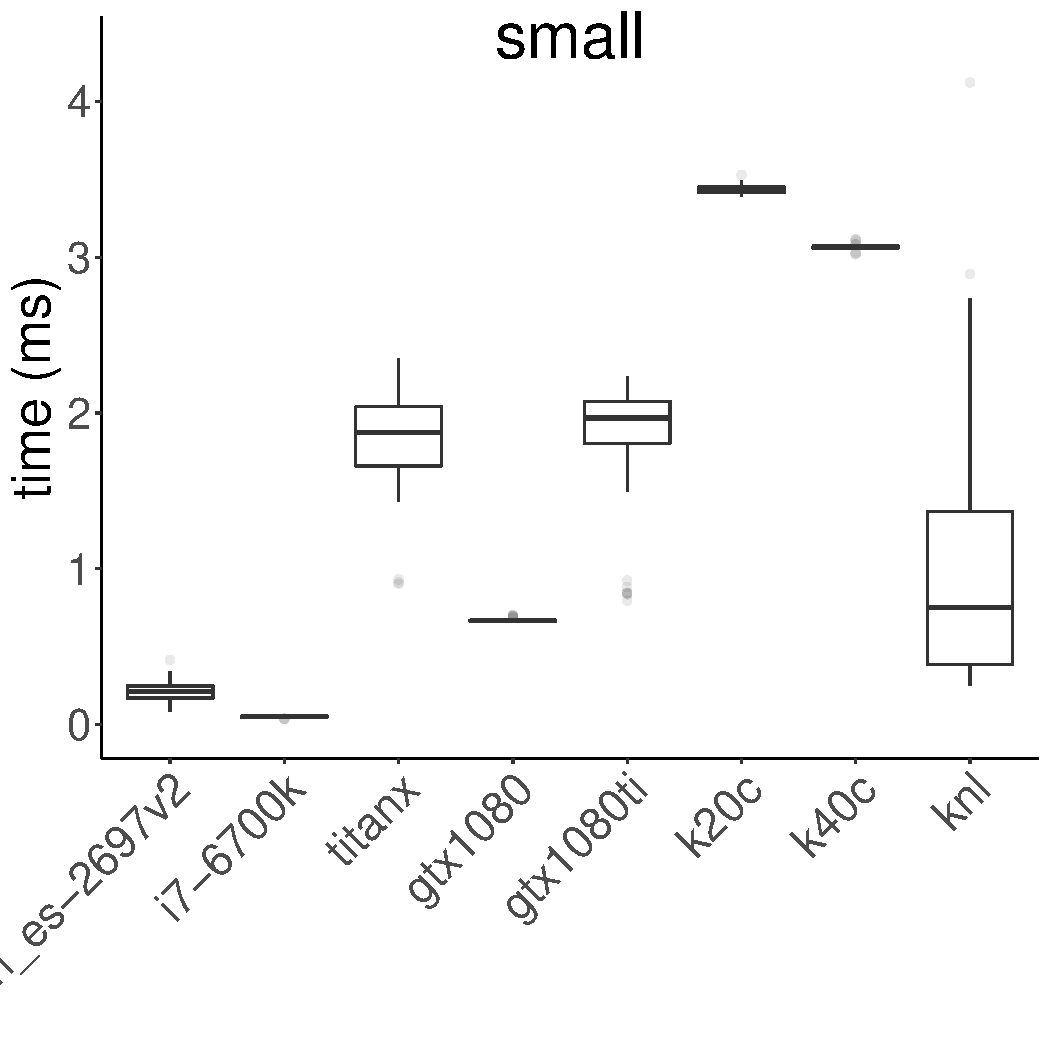
\includegraphics[width=0.23\textwidth]{figures/time-results/generate_crc_small_boxplot_knl-1}
	
	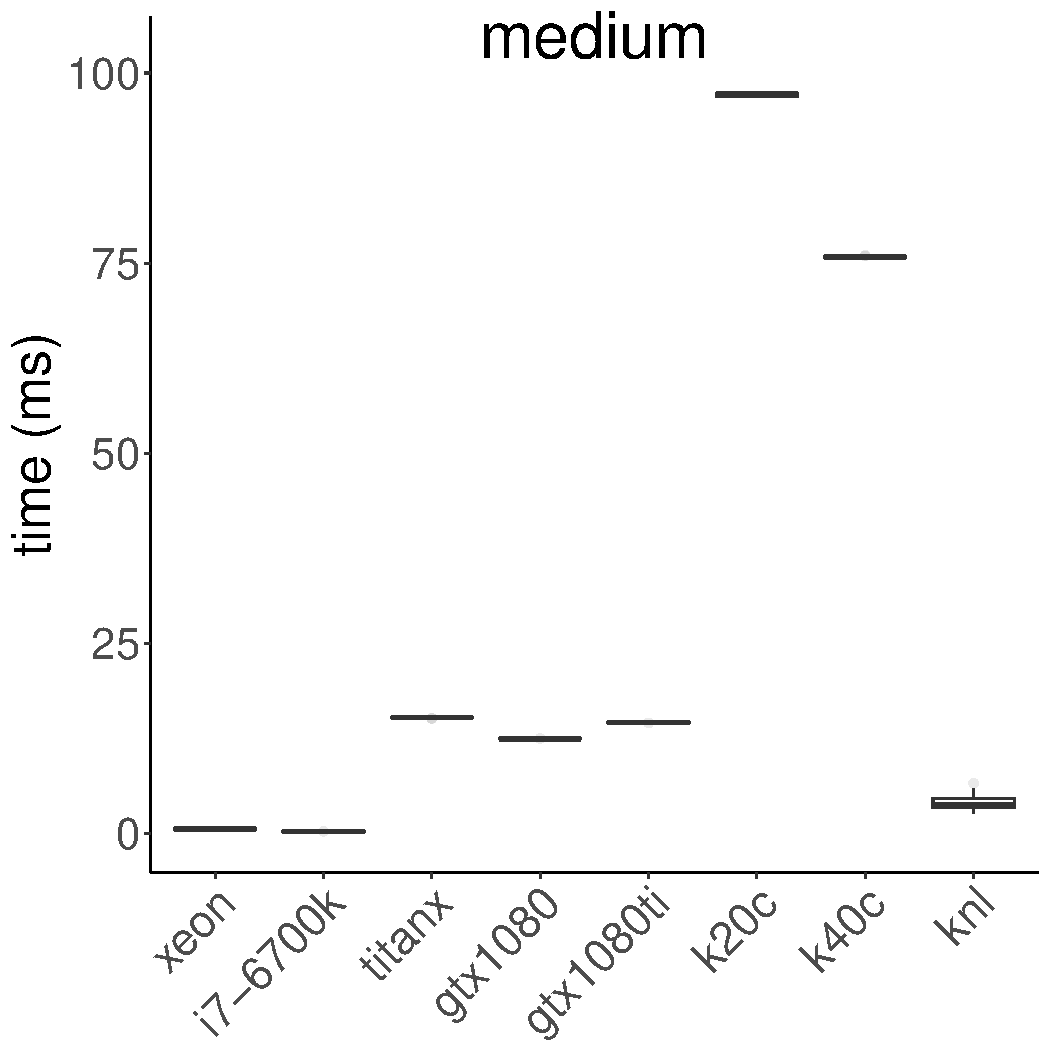
\includegraphics[width=0.23\textwidth]{figures/time-results/generate_crc_medium_boxplot_knl-1}
	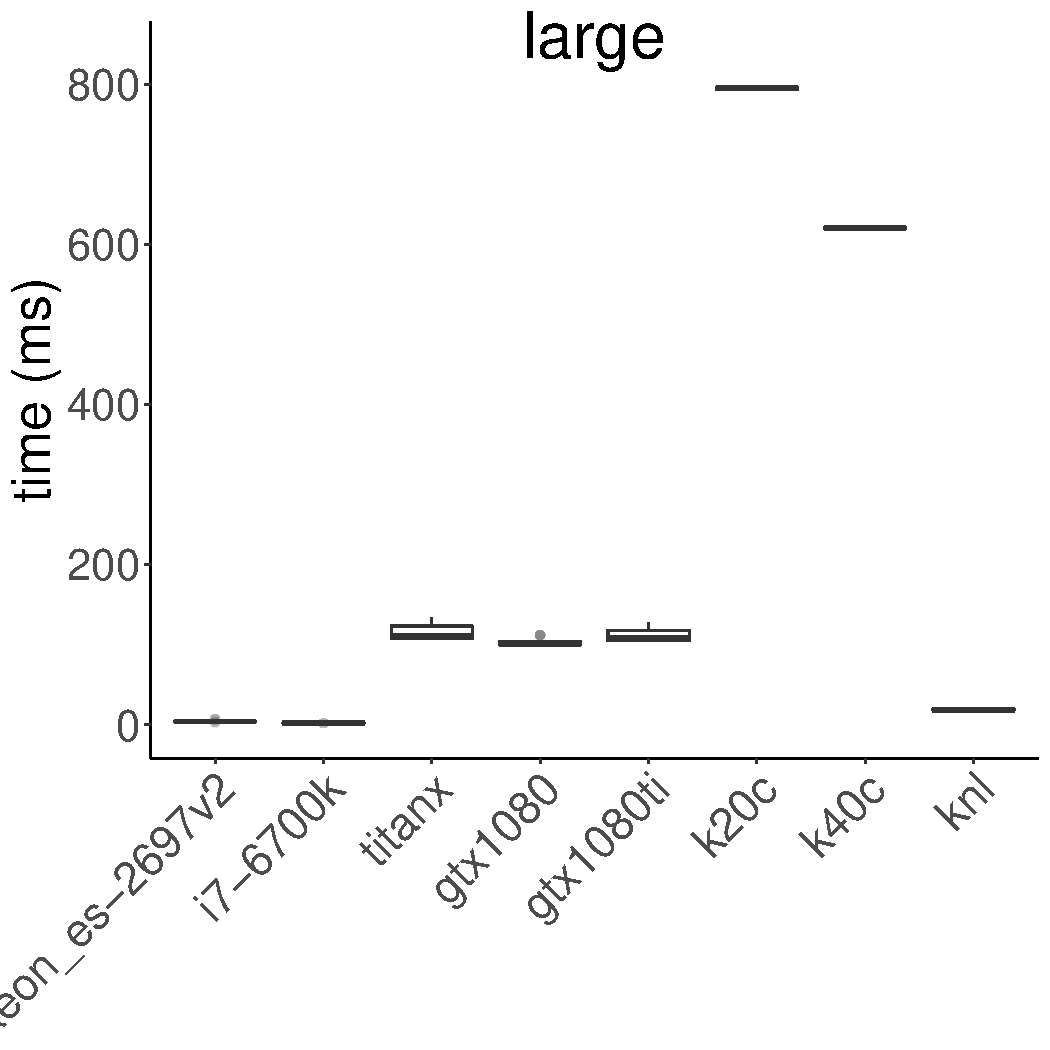
\includegraphics[width=0.23\textwidth]{figures/time-results/generate_crc_large_boxplot_knl-1}
	\caption{Kernel Execution times for {\bf crc}, the only application favouring the CPU architectures.}
	\label{fig:time-crc}
\end{figure}

Figure~\ref{fig:time} shows the distribution of execution times for the remaining benchmarks.
Each benchmark corresponds to a particular dwarf, Figure~\ref{fig:time-kmeans} and Figure~\ref{fig:time-lud} are both representative of the Dense Linear Algebra dwarf, Figure~\ref{fig:time-dwt} and Figure~\ref{fig:time-fft} are representative of Spectral Methods,
Figure~\ref{fig:time-gem} represents N-Body Methods, and Figure~\ref{fig:time-srad} represents the Structured Grid dwarf.

\captionsetup[subfigure]{justification=raggedright,singlelinecheck=false}

\newcommand{\plotwidth}{0.24\textwidth}
\begin{figure*}
	\begin{subfigure}{0.09\textwidth}\subcaption[l]{\bf kmeans} \label{fig:time-kmeans} \vspace{5mm}\end{subfigure}
	\begin{subfigure}{0.9\textwidth}
		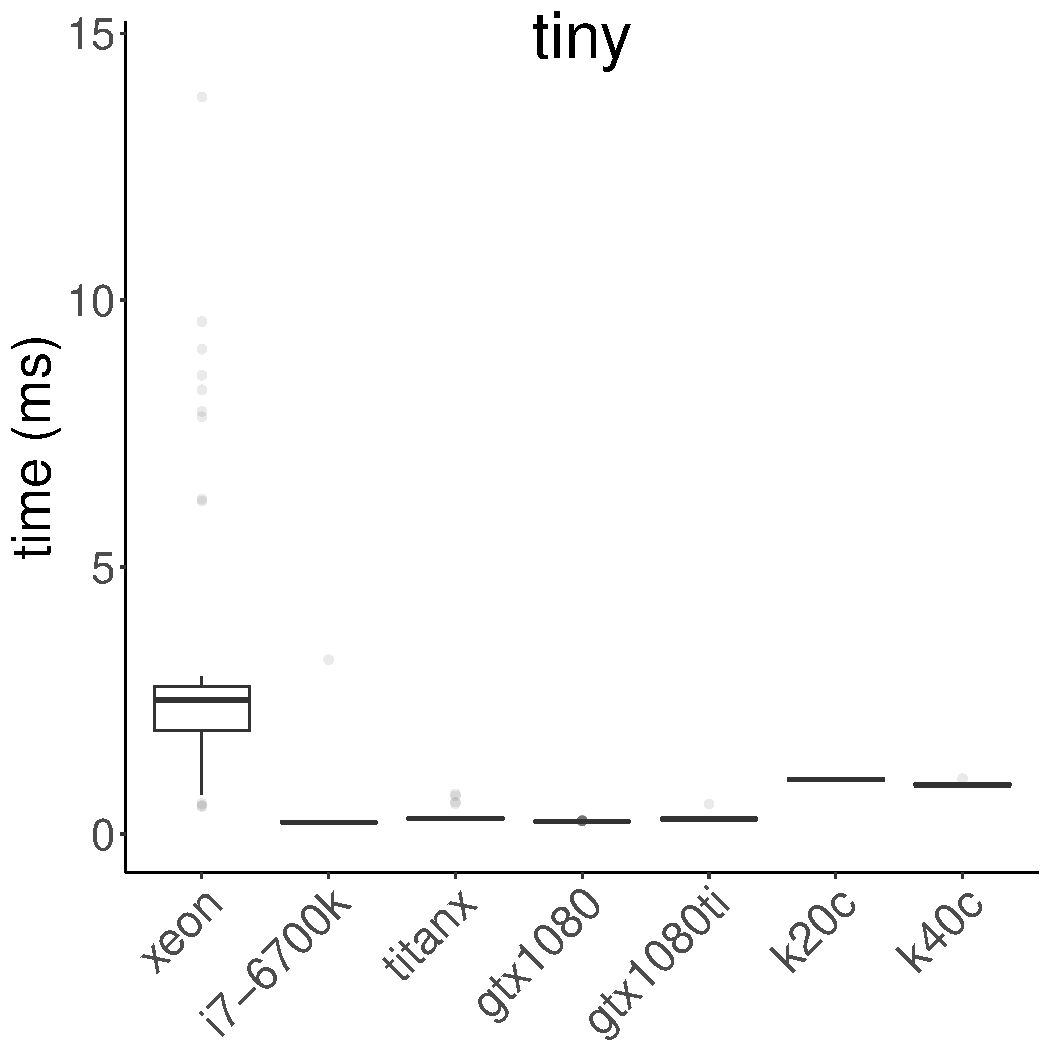
\includegraphics[width=\plotwidth]{figures/time-results/generate_kmeans_no_knl_tiny_boxplot-1}
		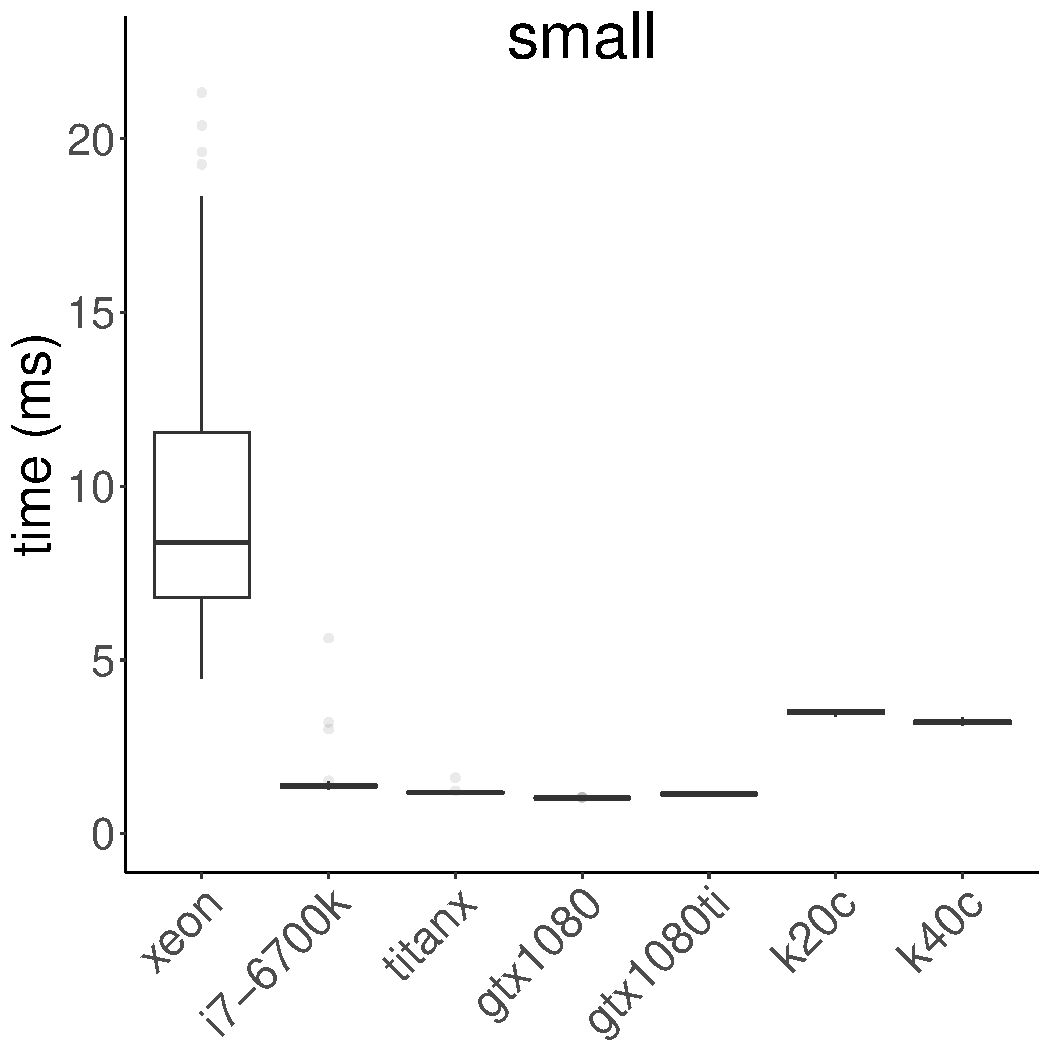
\includegraphics[width=\plotwidth]{figures/time-results/generate_kmeans_no_knl_small_boxplot-1}
		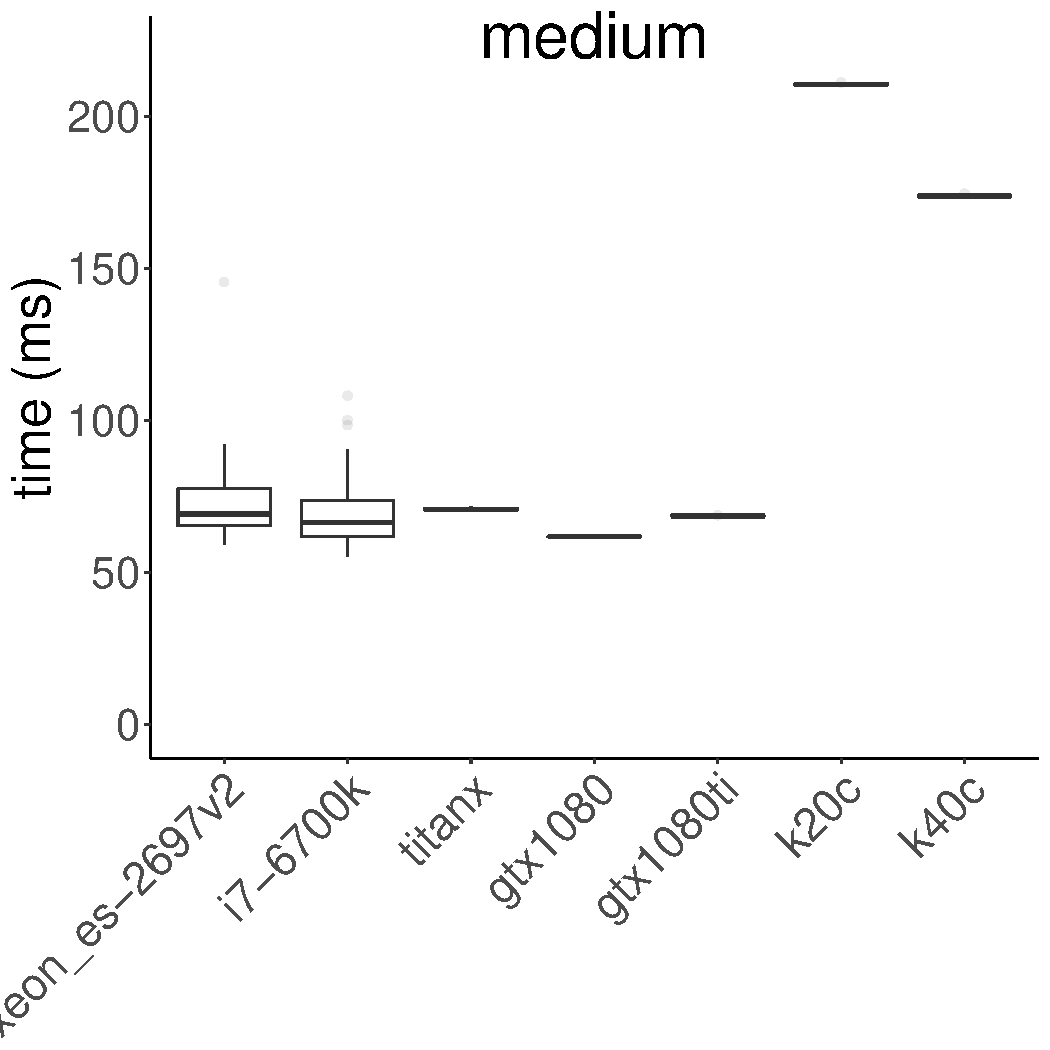
\includegraphics[width=\plotwidth]{figures/time-results/generate_kmeans_no_knl_medium_boxplot-1}
		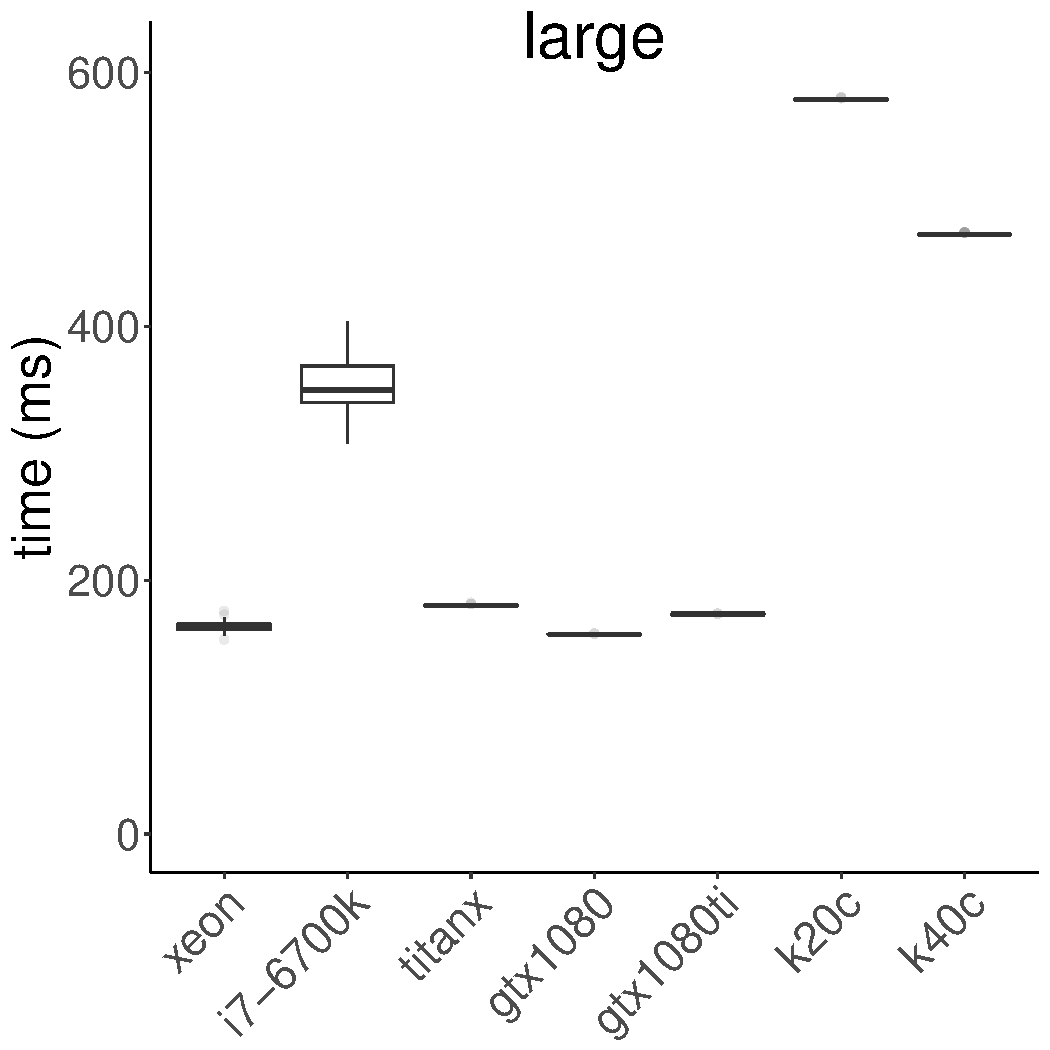
\includegraphics[width=\plotwidth]{figures/time-results/generate_kmeans_no_knl_large_boxplot-1}
	\end{subfigure}

	\begin{subfigure}{0.09\textwidth}\subcaption[l]{\bf lud} \label{fig:time-lud} \vspace{5mm}\end{subfigure}
	\begin{subfigure}{0.9\textwidth}
		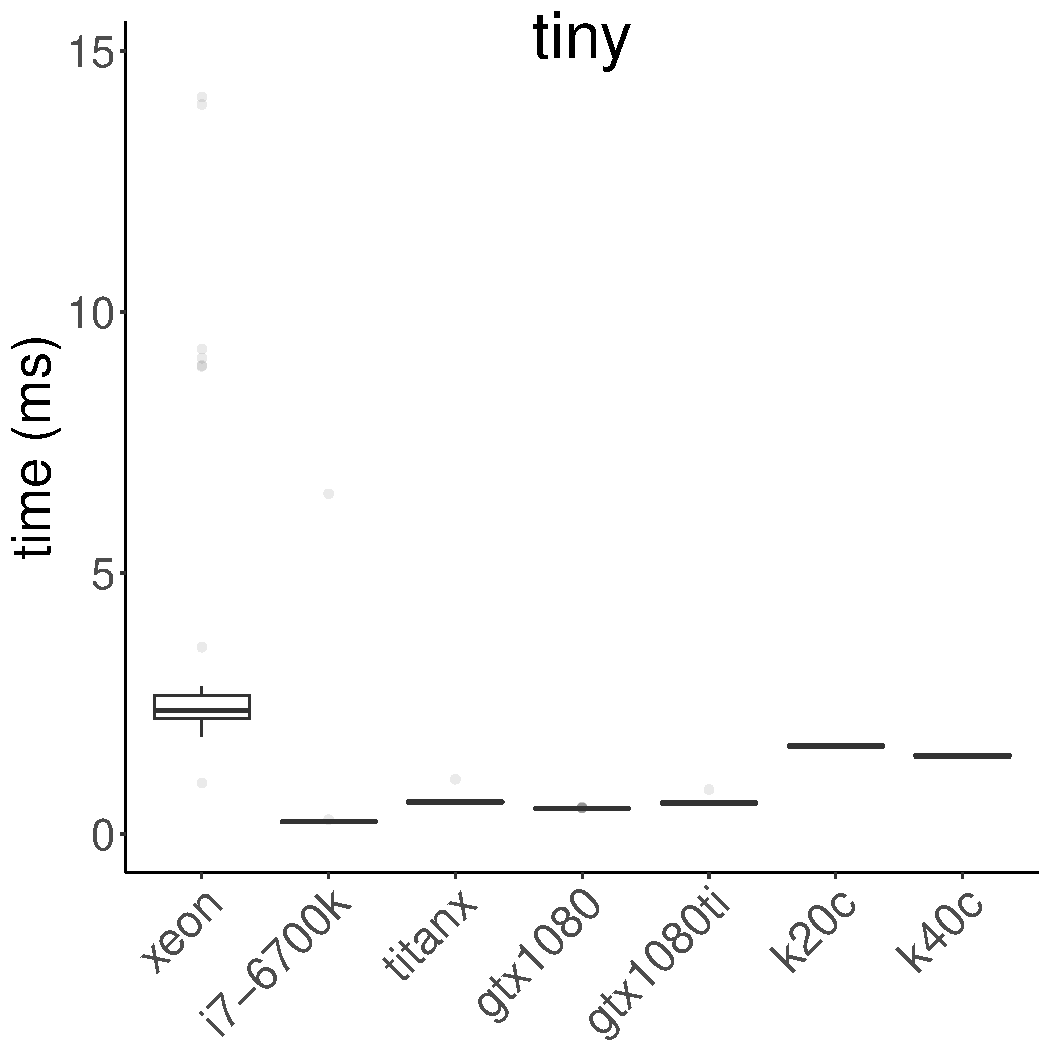
\includegraphics[width=\plotwidth]{figures/time-results/generate_lud_tiny_boxplot-1}
		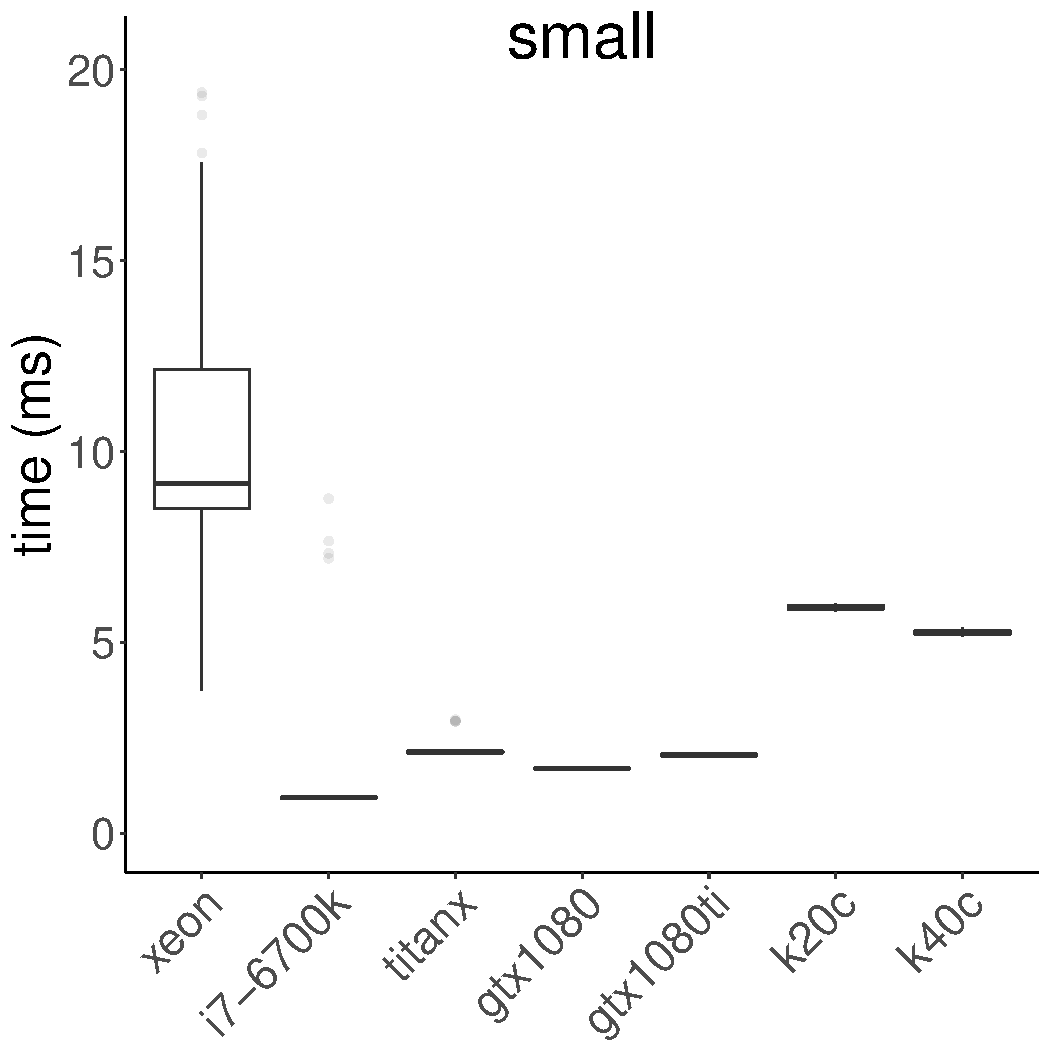
\includegraphics[width=\plotwidth]{figures/time-results/generate_lud_small_boxplot-1}
		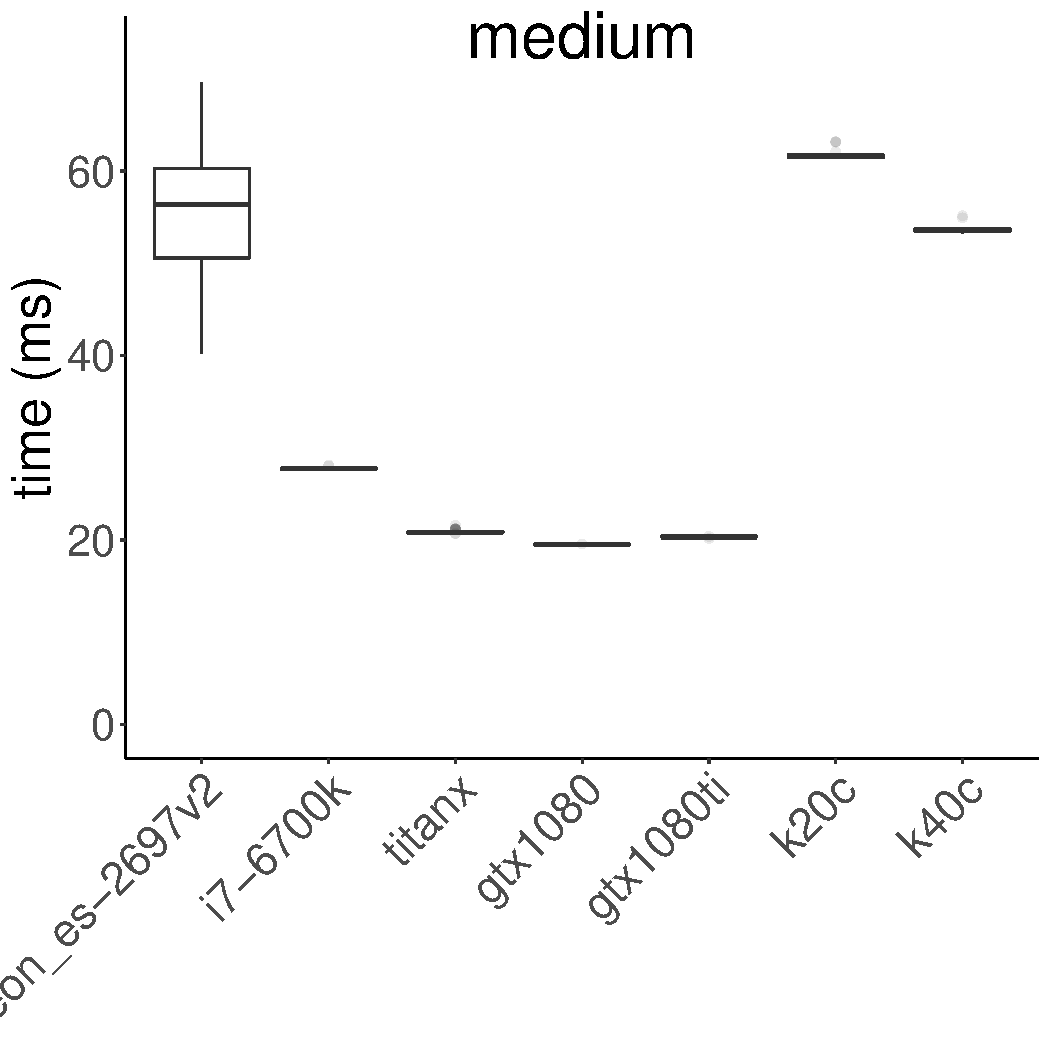
\includegraphics[width=\plotwidth]{figures/time-results/generate_lud_medium_boxplot-1}
		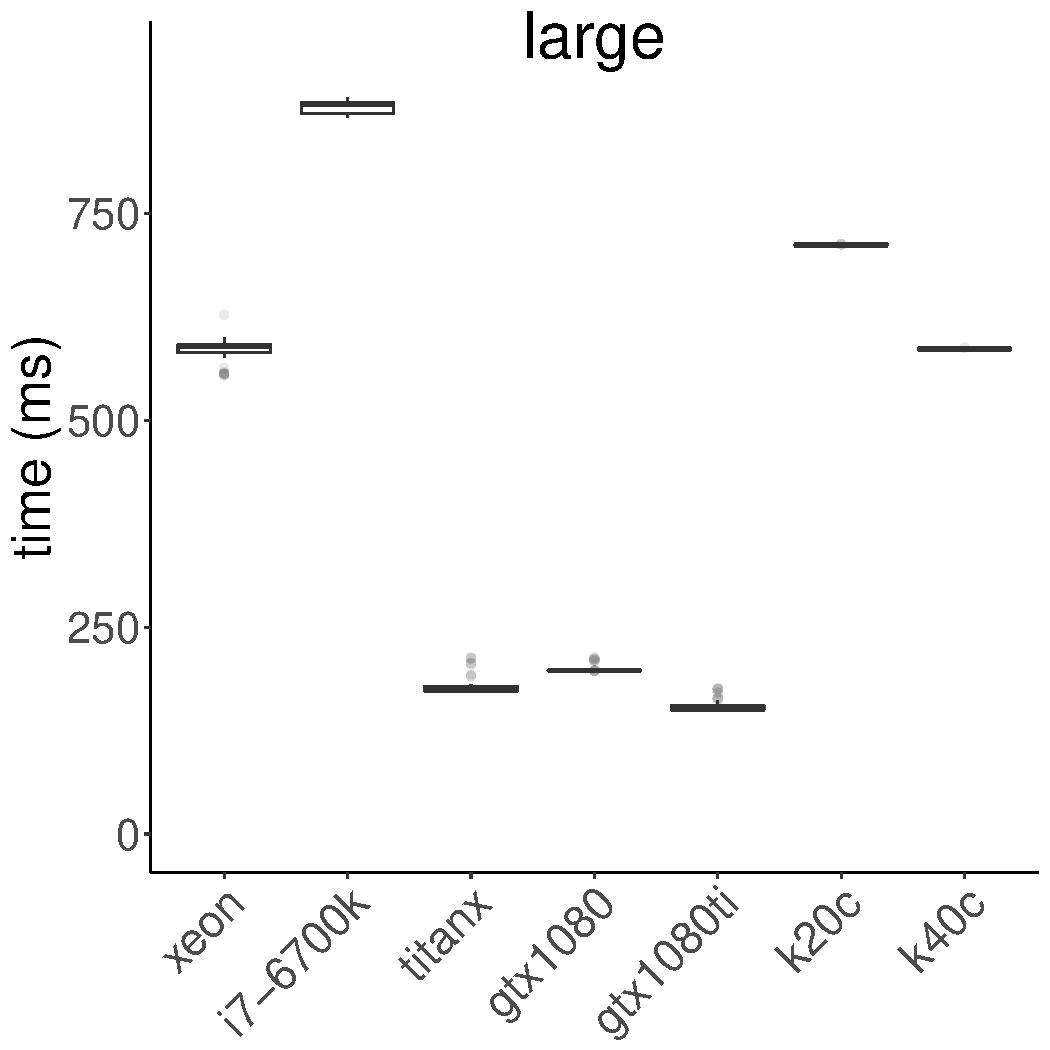
\includegraphics[width=\plotwidth]{figures/time-results/generate_lud_large_boxplot-1}
	\end{subfigure}
	
	\begin{subfigure}{0.09\textwidth}\subcaption[l]{\bf dwt} \label{fig:time-dwt} \vspace{5mm}\end{subfigure}
	\begin{subfigure}{0.9\textwidth}
		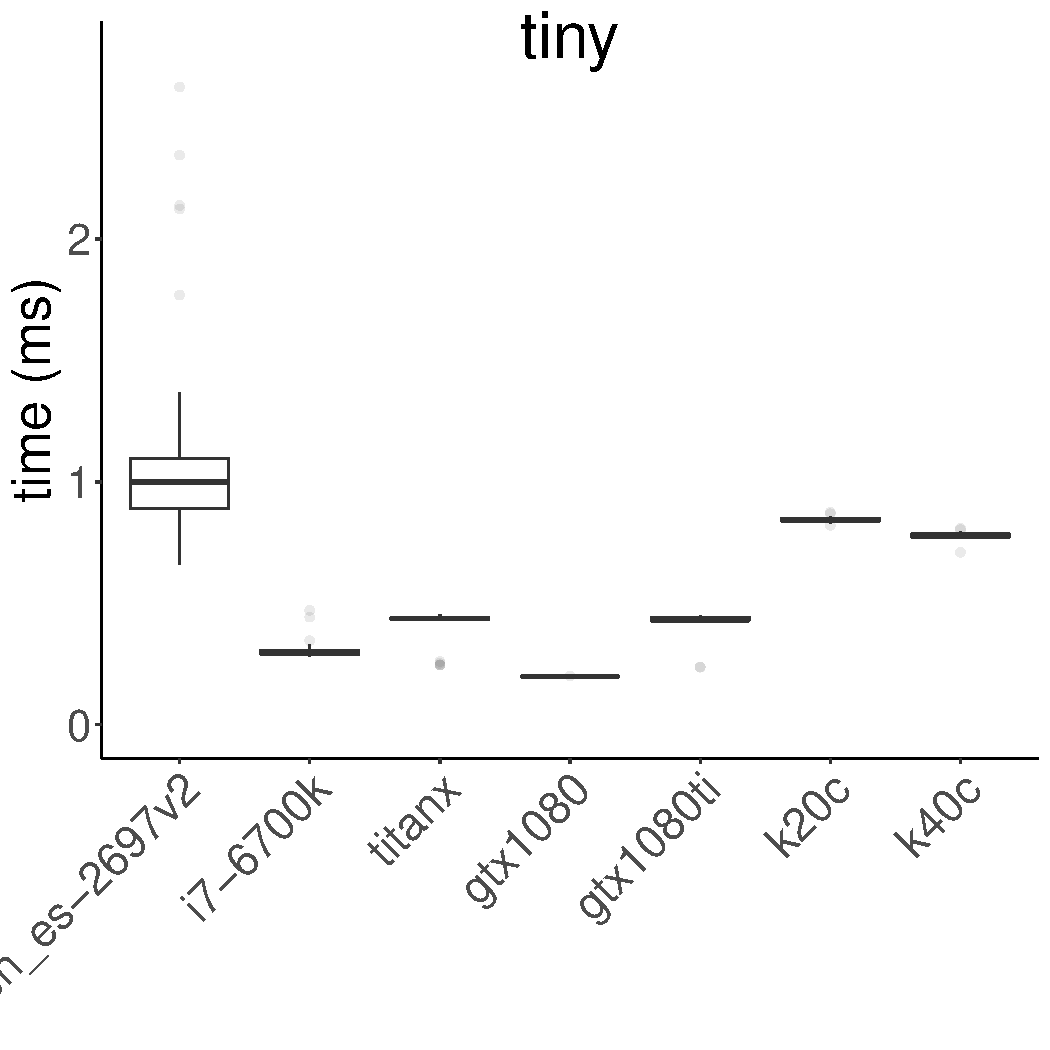
\includegraphics[width=\plotwidth]{figures/time-results/generate_dwt_tiny_boxplot-1}
		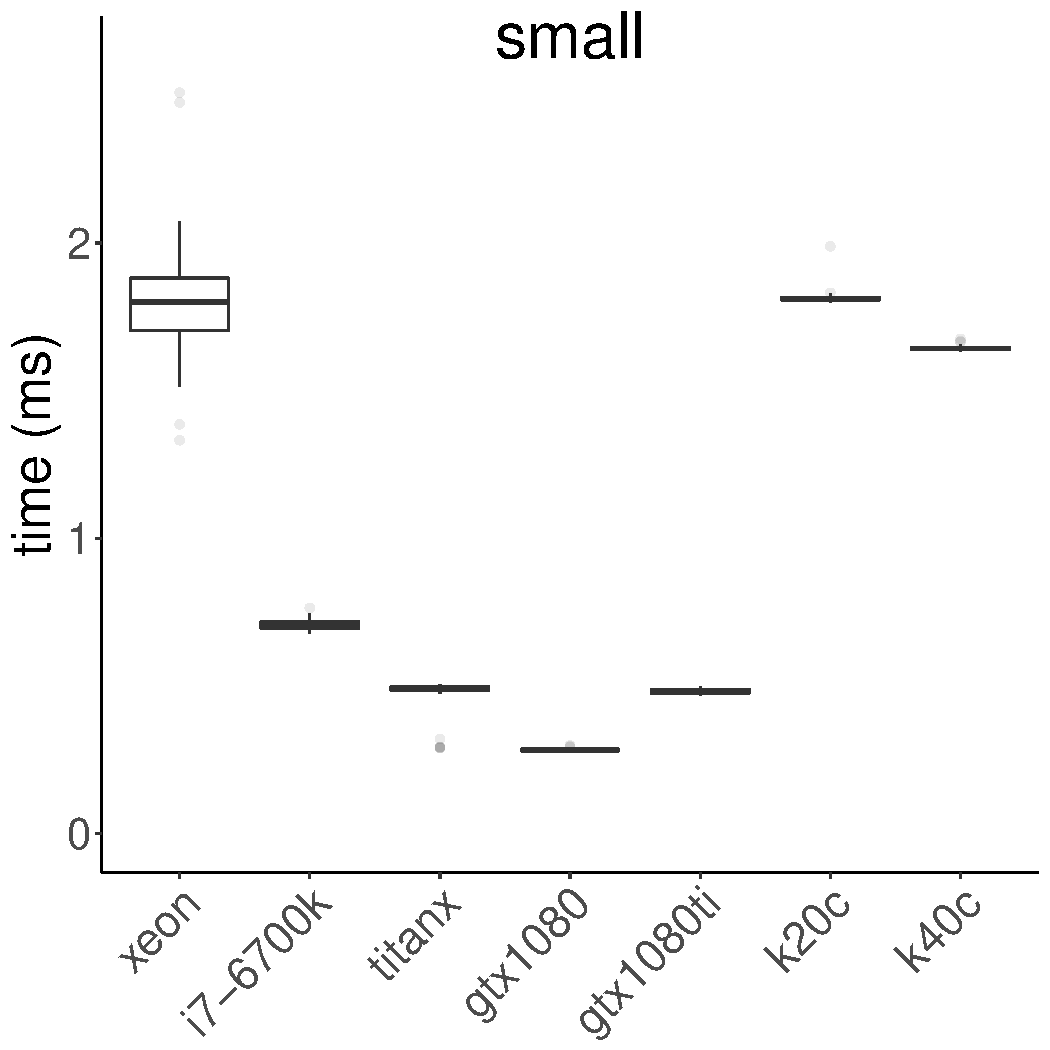
\includegraphics[width=\plotwidth]{figures/time-results/generate_dwt_small_boxplot-1}
		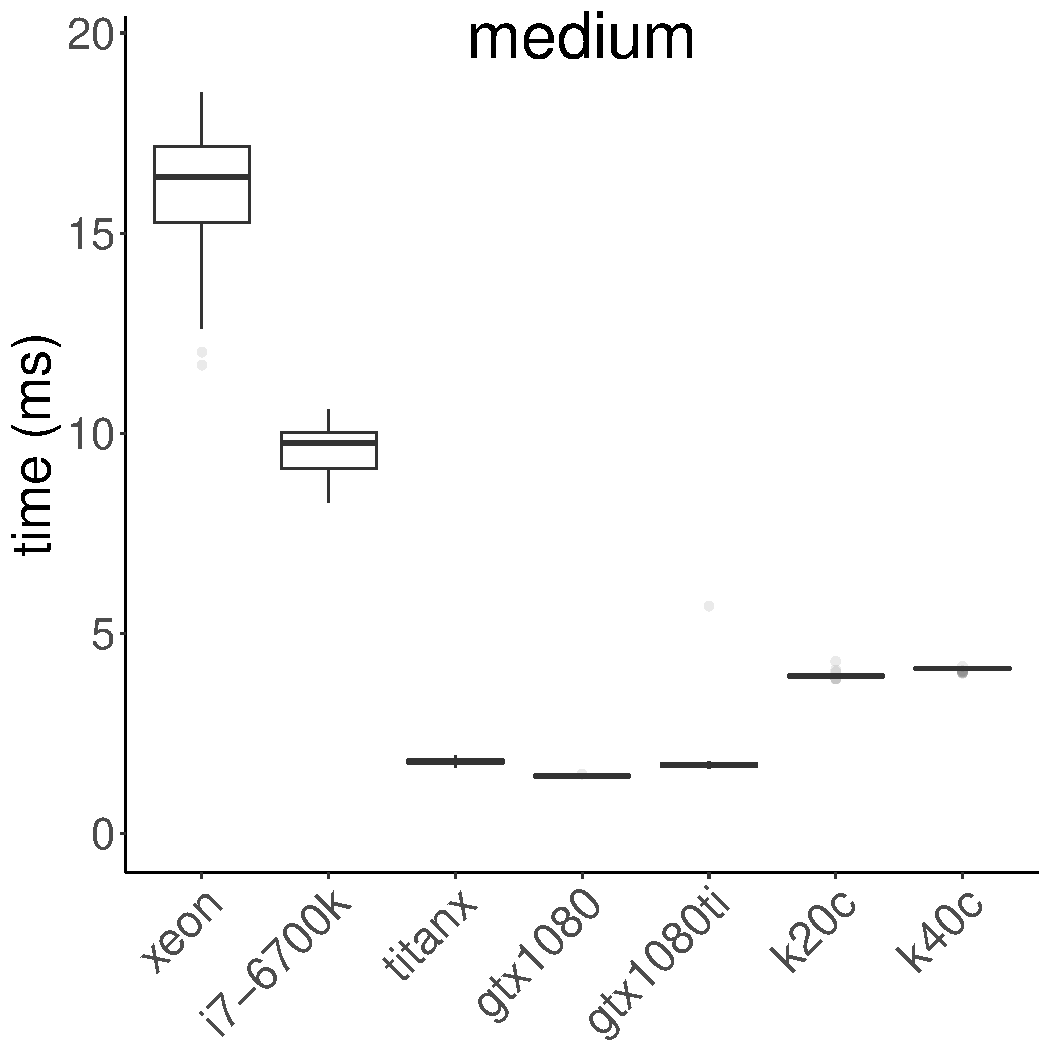
\includegraphics[width=\plotwidth]{figures/time-results/generate_dwt_medium_boxplot-1}
		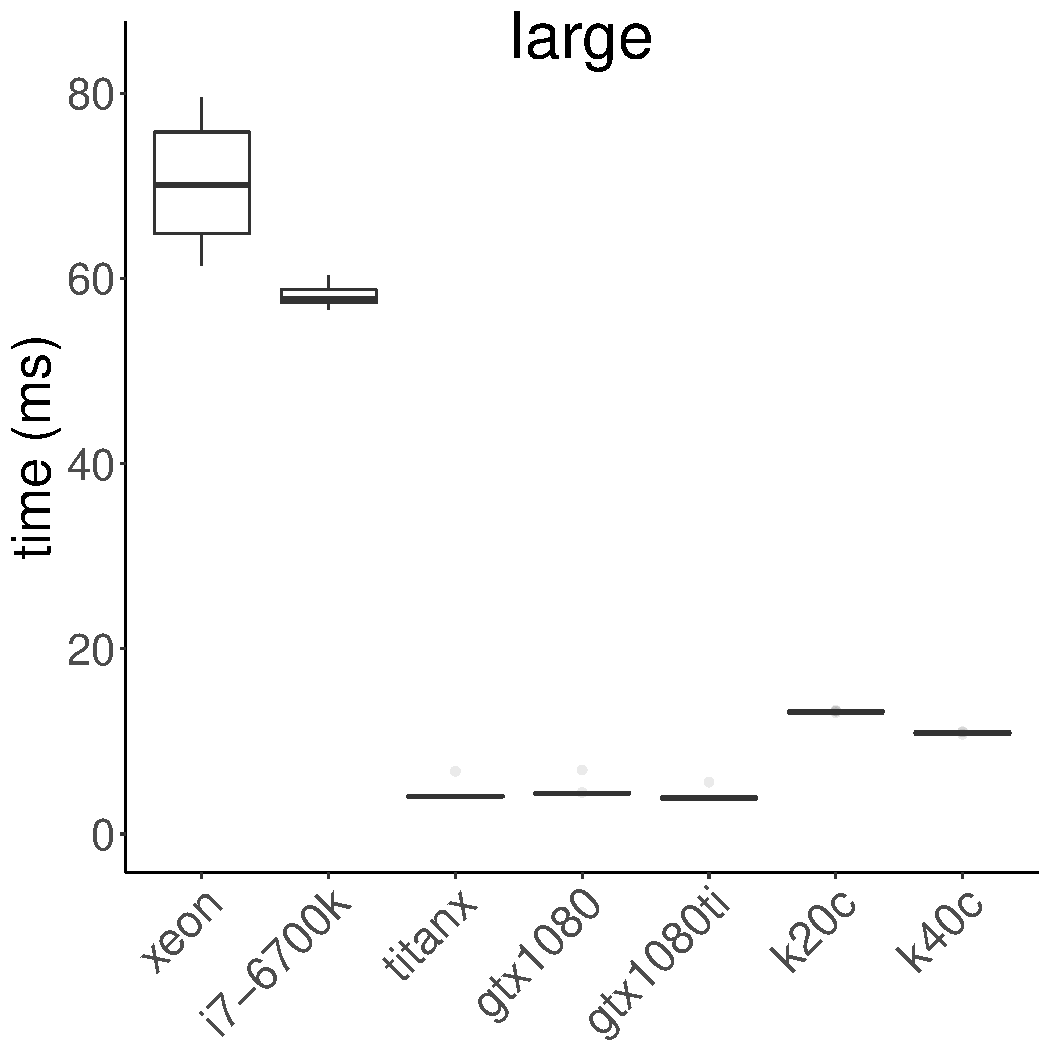
\includegraphics[width=\plotwidth]{figures/time-results/generate_dwt_large_boxplot-1}
	\end{subfigure}

	\begin{subfigure}{0.09\textwidth}\subcaption[l]{\bf fft} \label{fig:time-fft} \vspace{5mm}\end{subfigure}
	\begin{subfigure}{0.9\textwidth}
		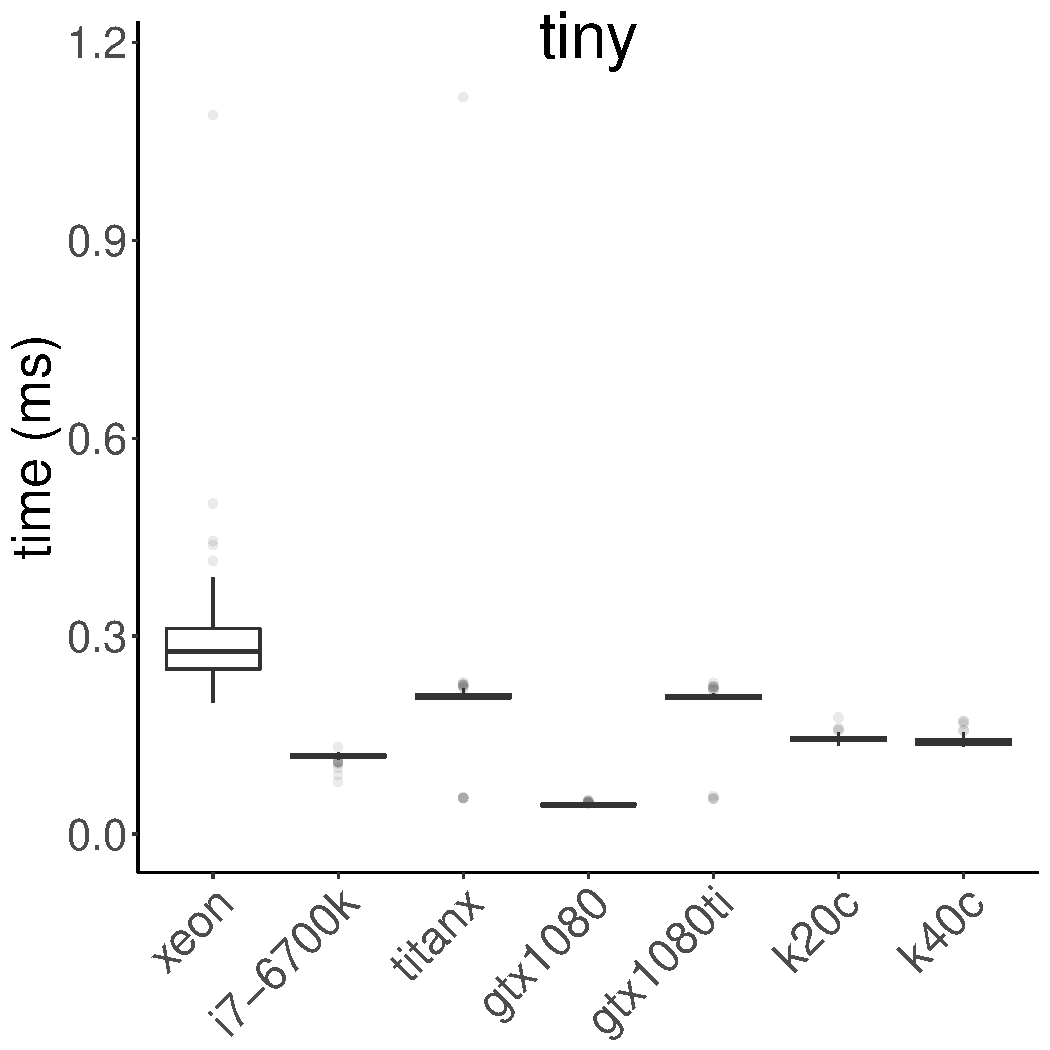
\includegraphics[width=\plotwidth]{figures/time-results/generate_fft_tiny_boxplot-1}
		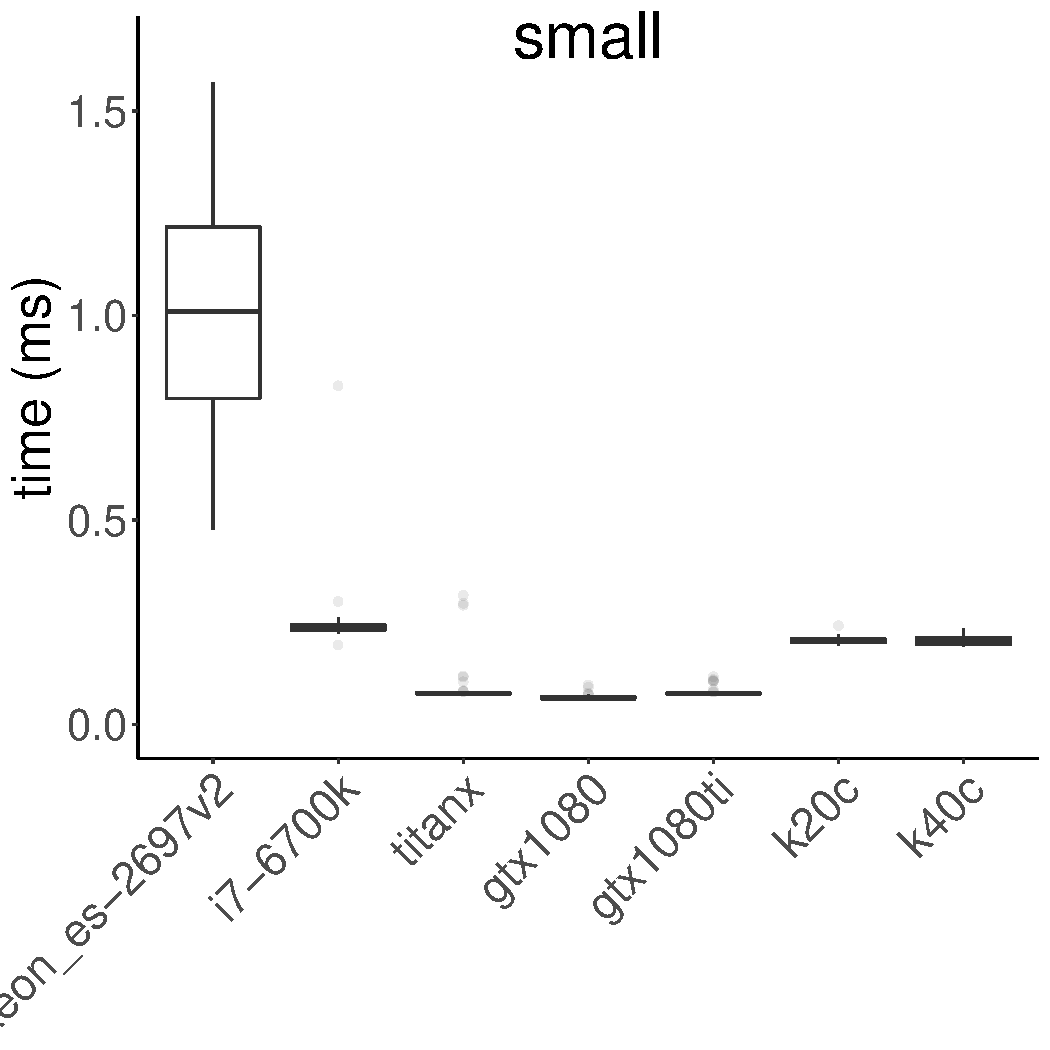
\includegraphics[width=\plotwidth]{figures/time-results/generate_fft_small_boxplot-1}
		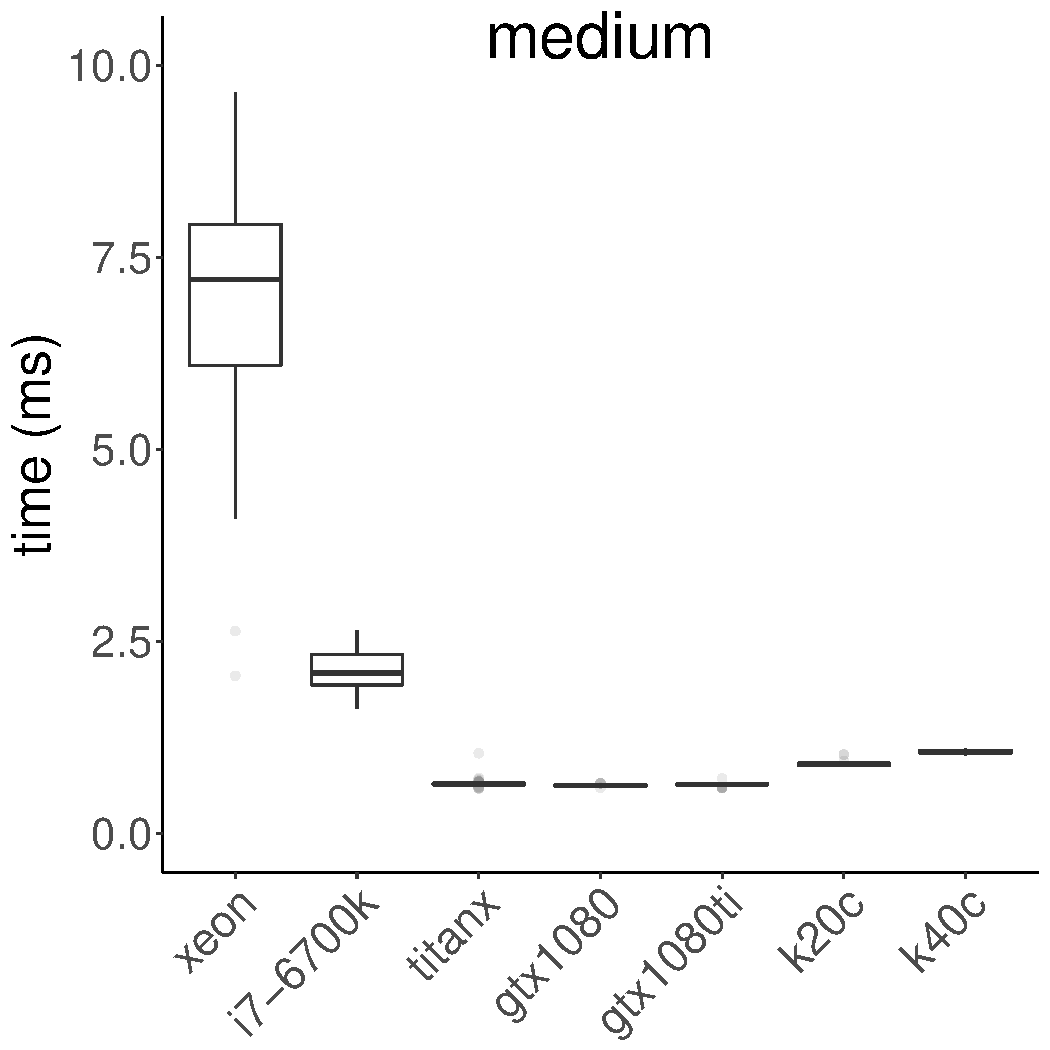
\includegraphics[width=\plotwidth]{figures/time-results/generate_fft_medium_boxplot-1}
		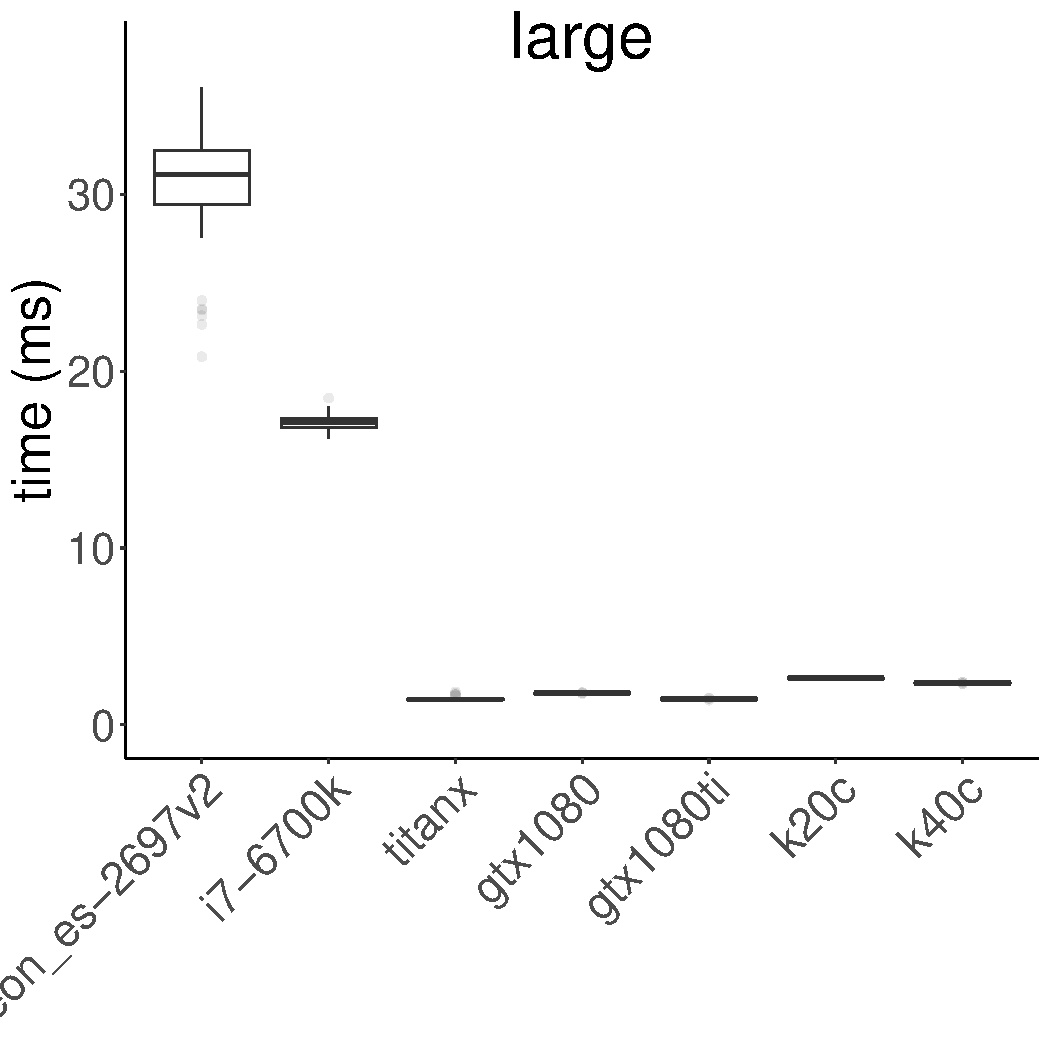
\includegraphics[width=\plotwidth]{figures/time-results/generate_fft_large_boxplot-1}
		\end{subfigure}

	\begin{subfigure}{0.09\textwidth}\subcaption[l]{\bf gem} \label{fig:time-gem} \vspace{5mm}\end{subfigure}
	\begin{subfigure}{0.9\textwidth}
		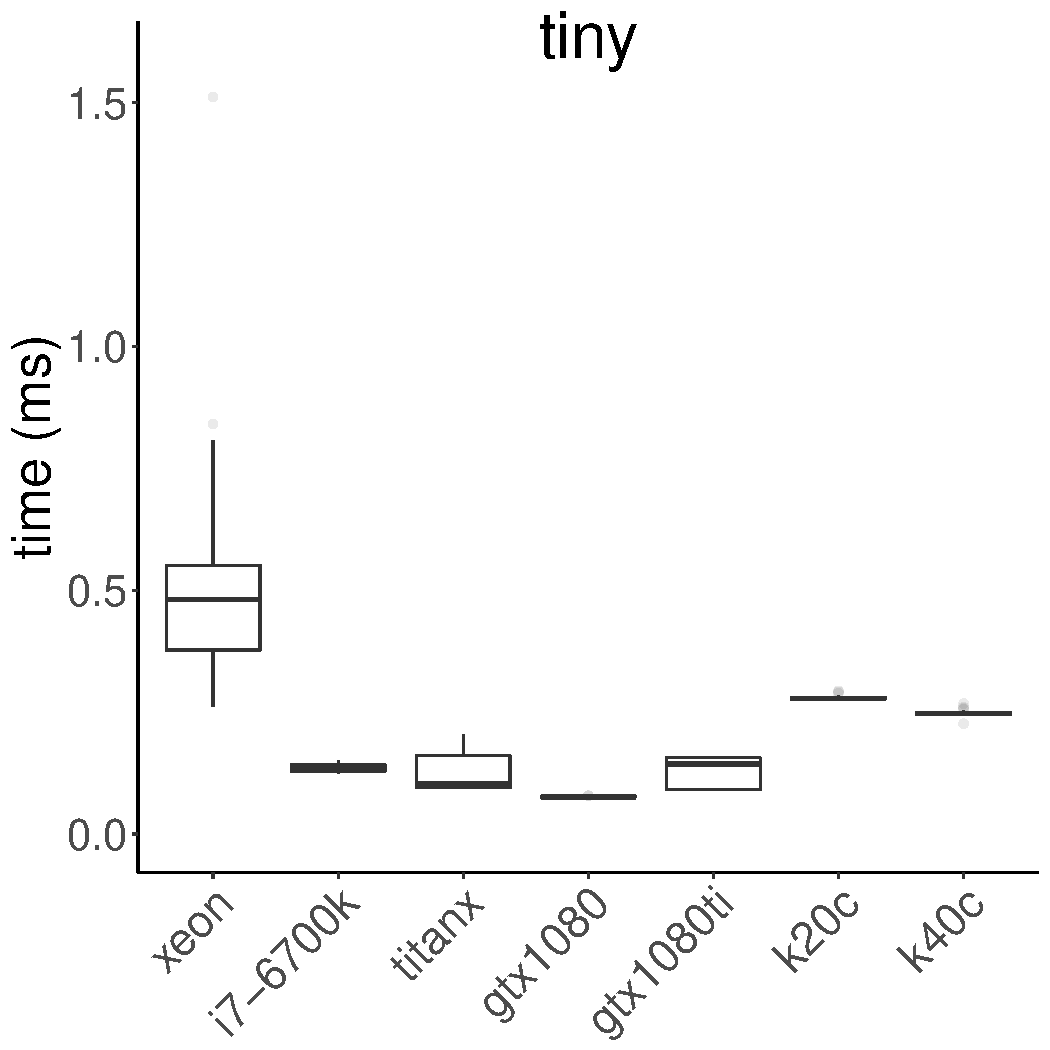
\includegraphics[width=\plotwidth]{figures/time-results/generate_gem_tiny_boxplot-1}
		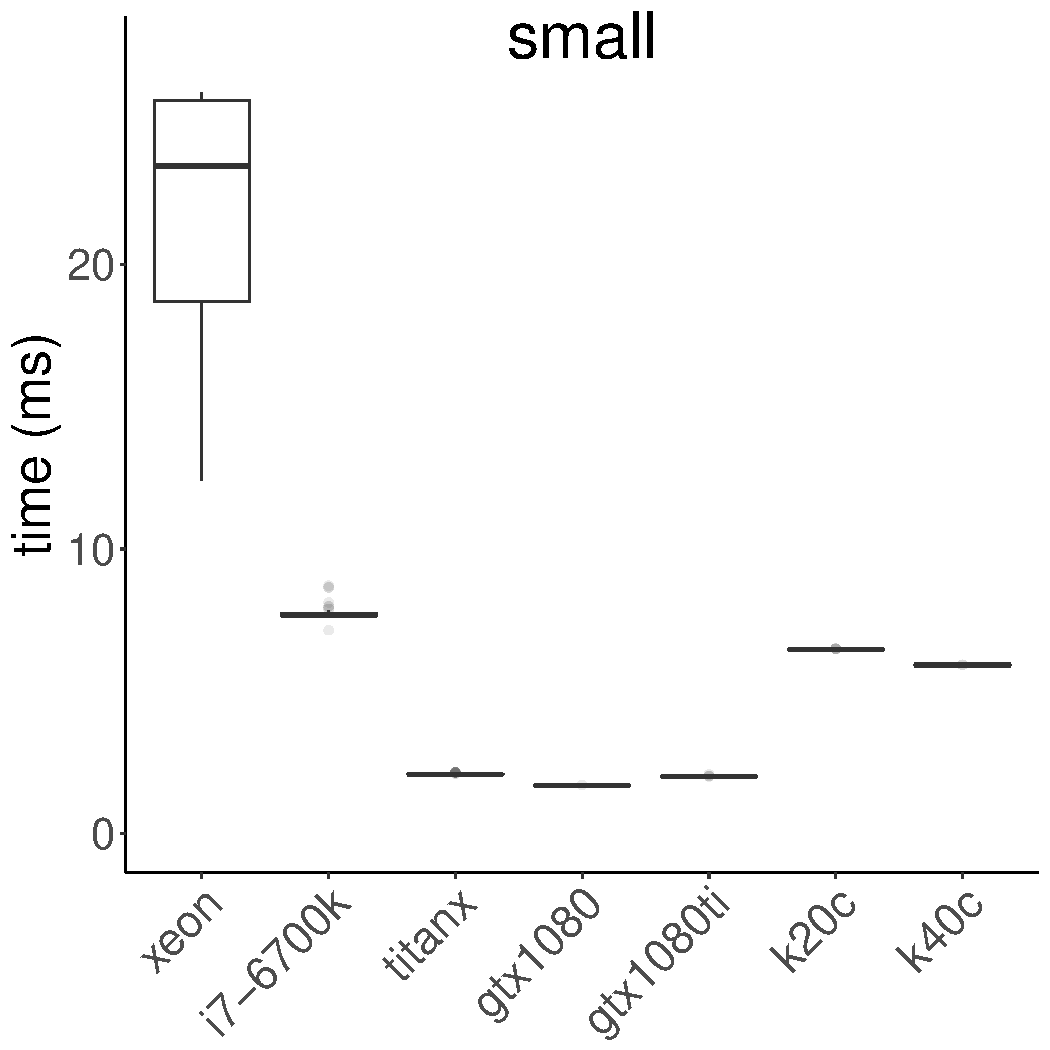
\includegraphics[width=\plotwidth]{figures/time-results/generate_gem_small_boxplot-1}
		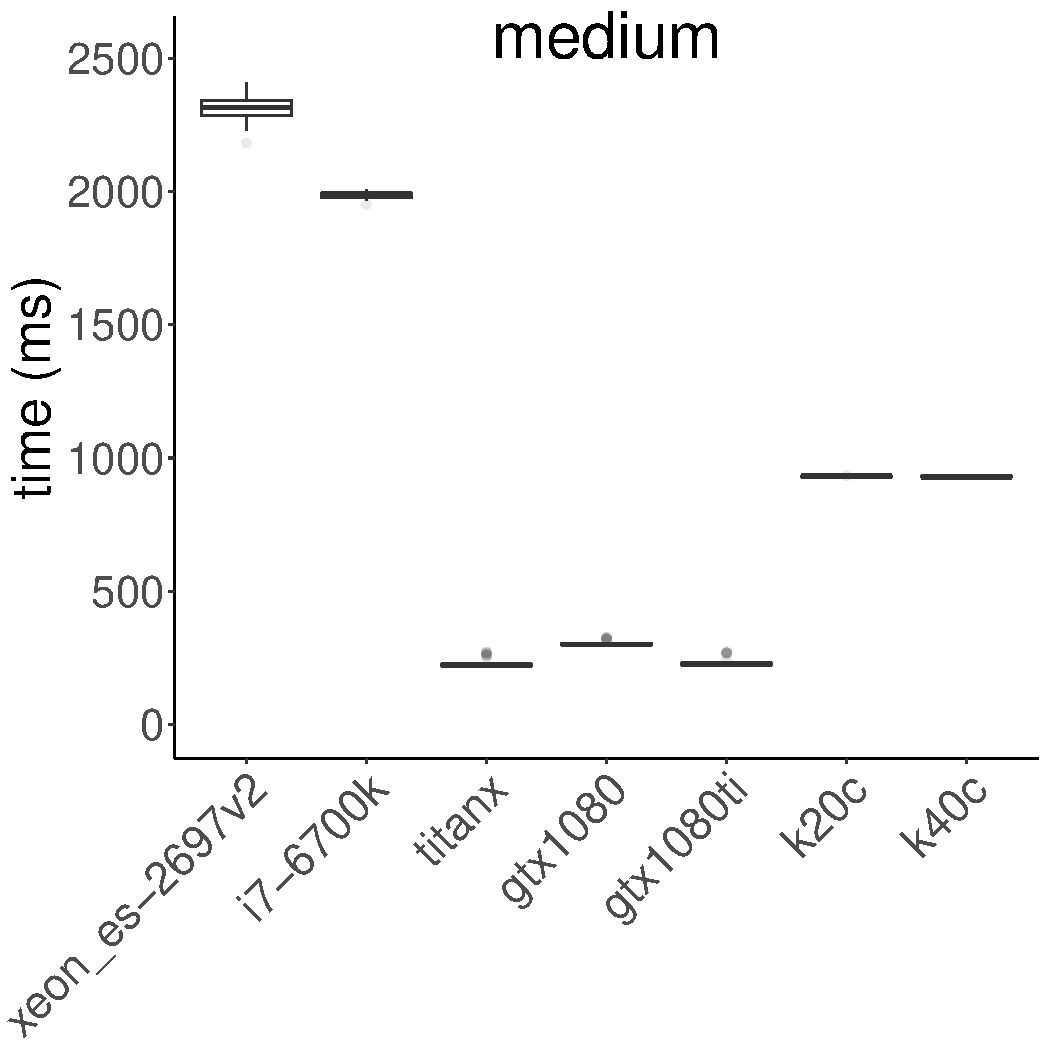
\includegraphics[width=\plotwidth]{figures/time-results/generate_gem_medium_boxplot-1}
		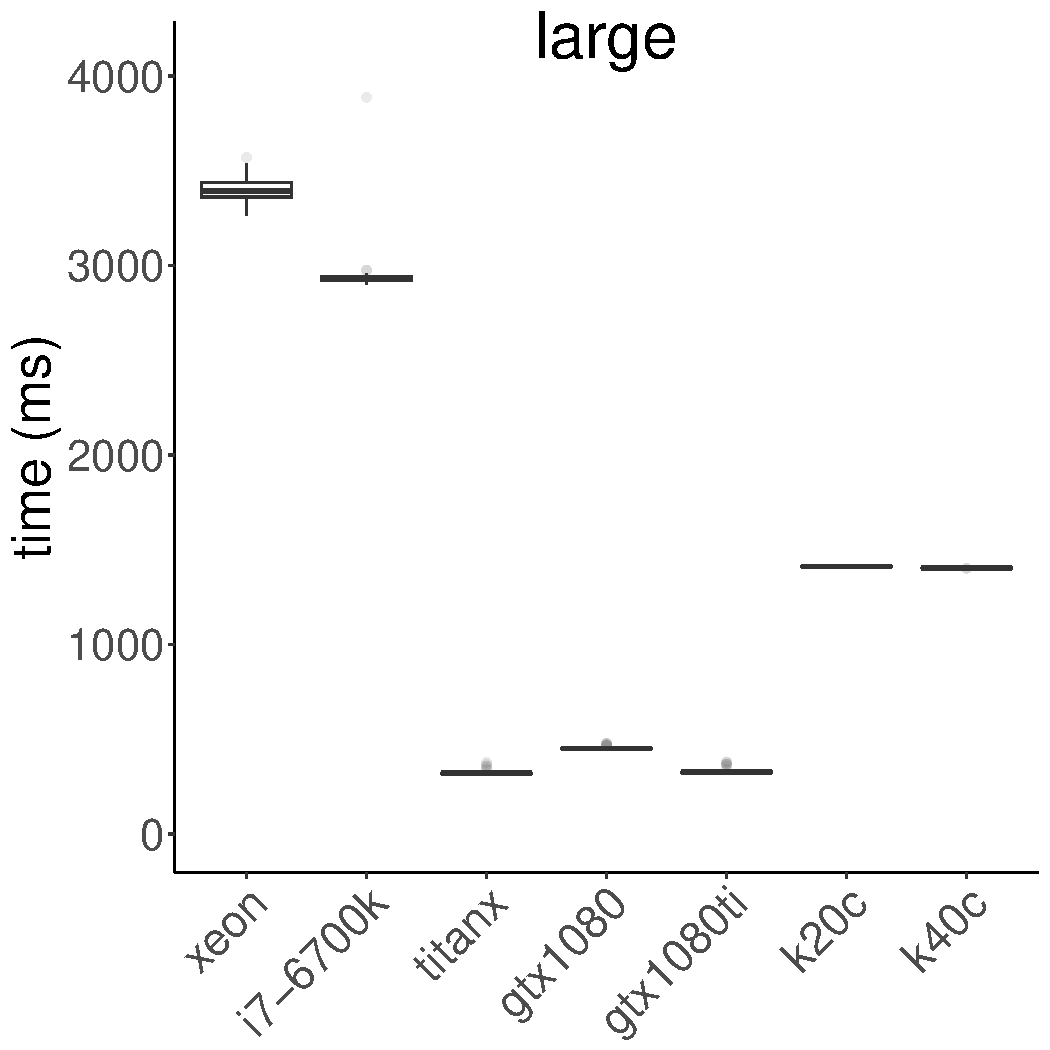
\includegraphics[width=\plotwidth]{figures/time-results/generate_gem_large_boxplot-1}
		\end{subfigure}

	\begin{subfigure}{0.09\textwidth}\subcaption[l]{\bf srad} \label{fig:time-srad} \vspace{5mm}\end{subfigure}
	\begin{subfigure}{0.9\textwidth}
		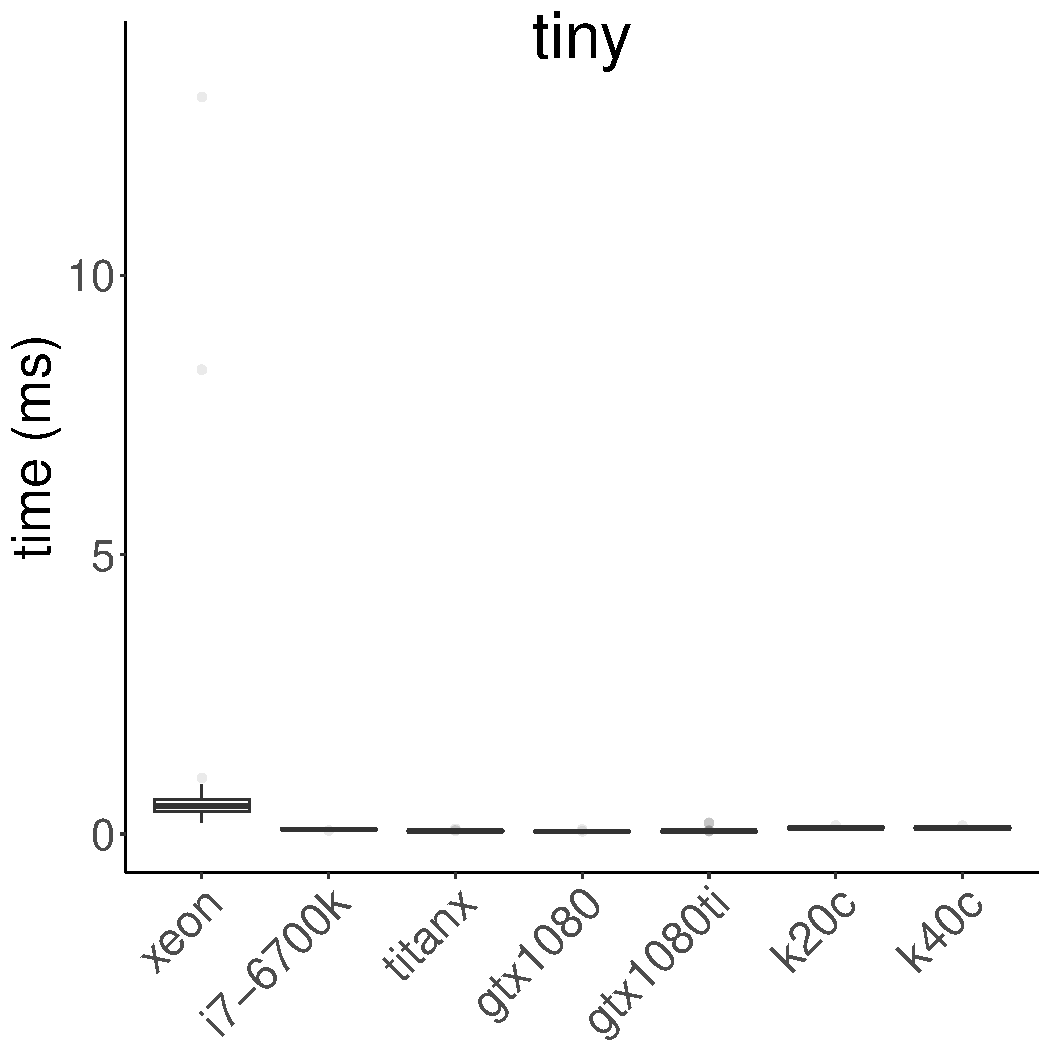
\includegraphics[width=\plotwidth]{figures/time-results/generate_srad_tiny_boxplot-1}
		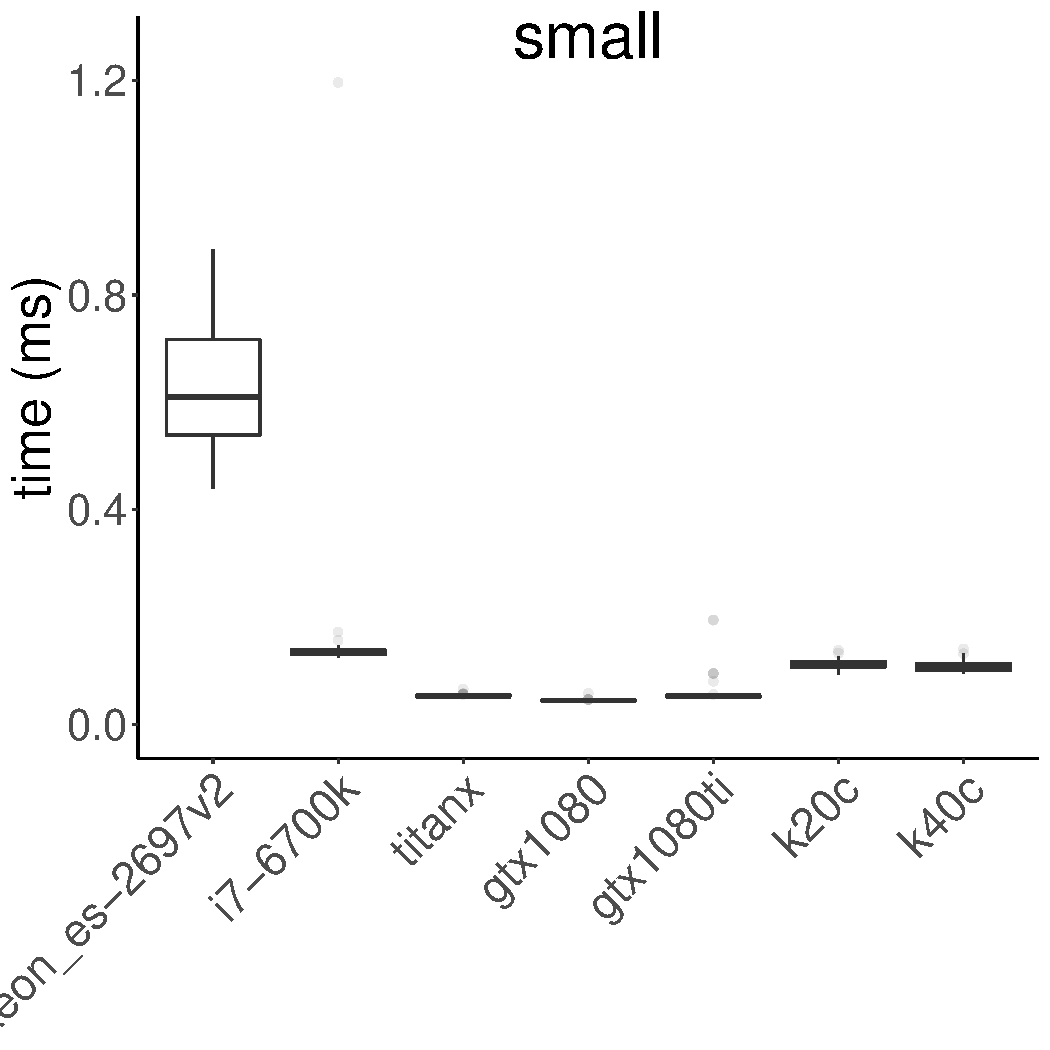
\includegraphics[width=\plotwidth]{figures/time-results/generate_srad_small_boxplot-1}
		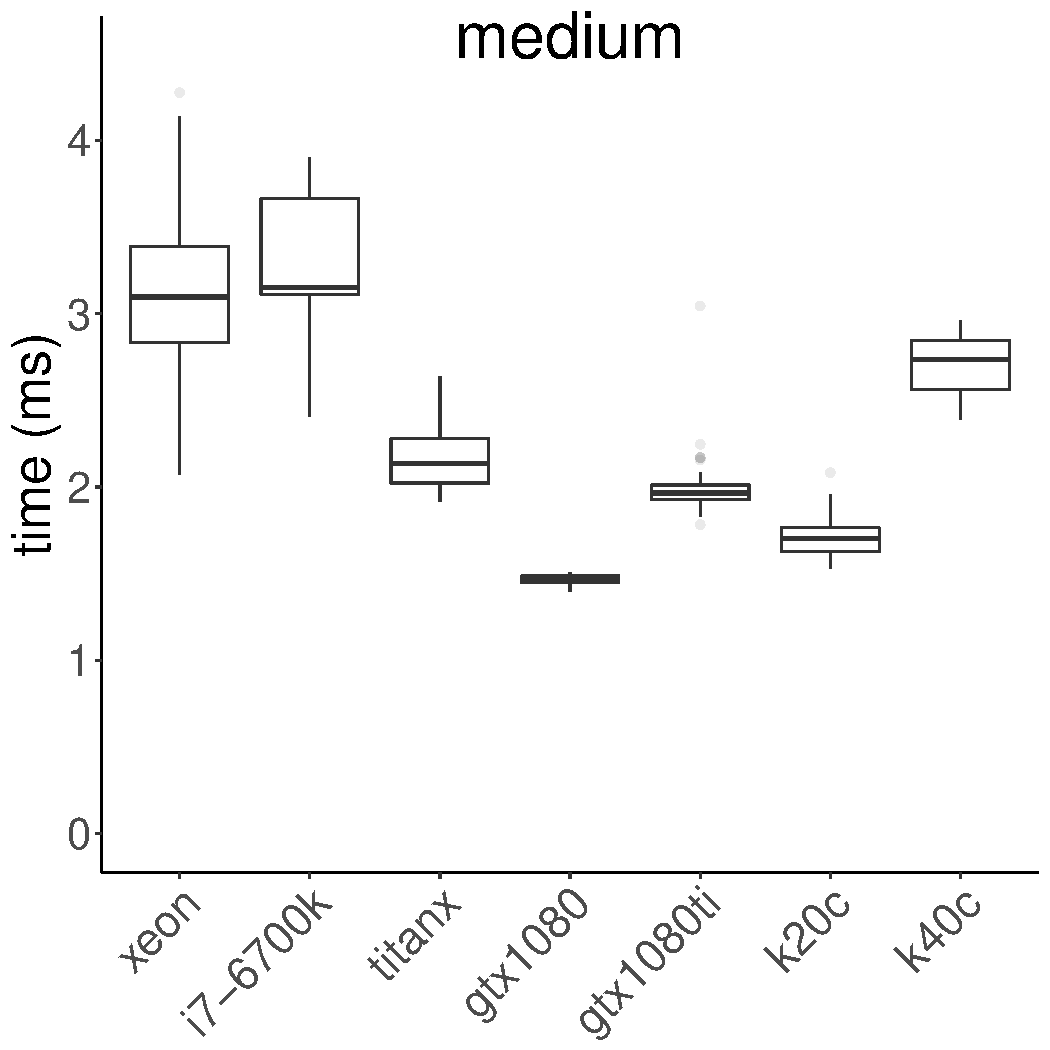
\includegraphics[width=\plotwidth]{figures/time-results/generate_srad_medium_boxplot-1}
		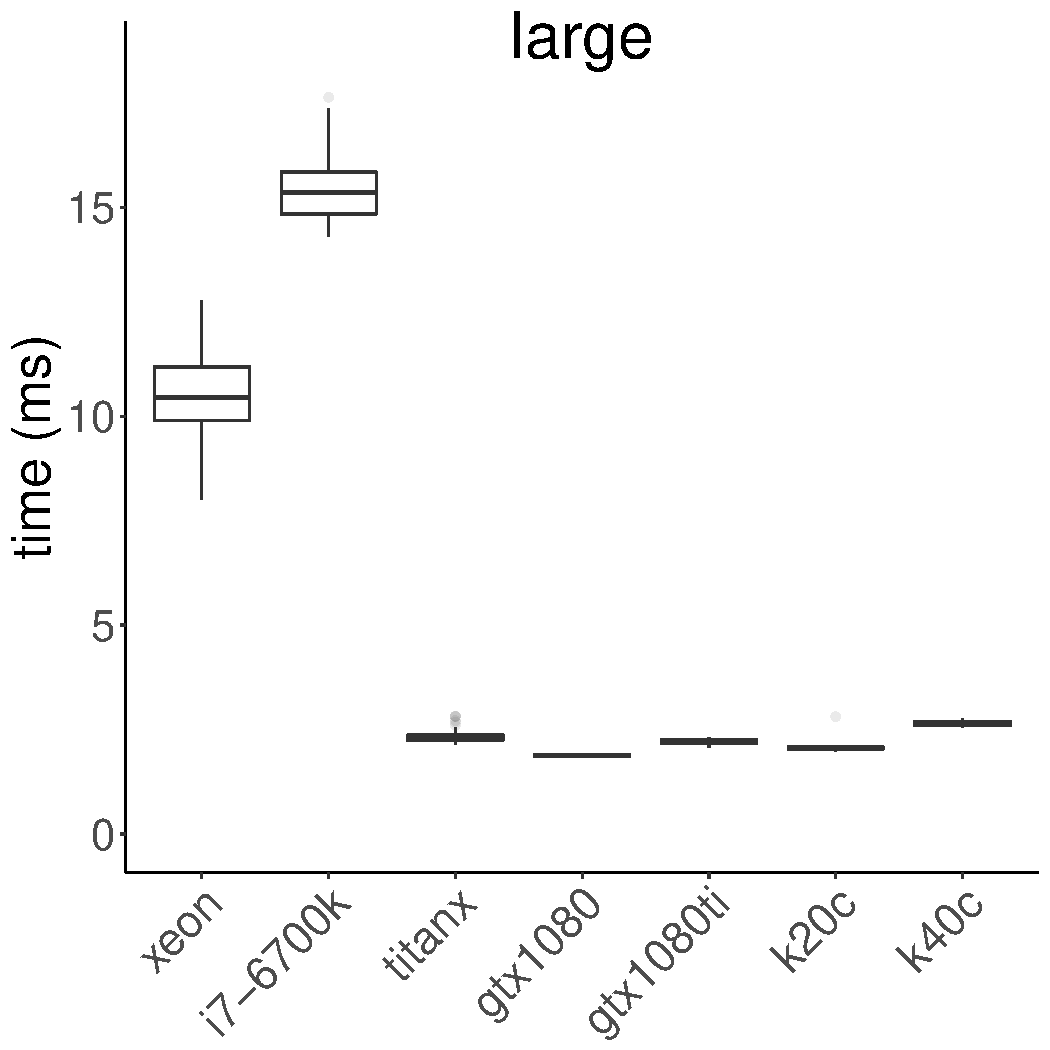
\includegraphics[width=\plotwidth]{figures/time-results/generate_srad_large_boxplot-1}
	\end{subfigure}
    \caption{Kernel execution times for benchmarks for which the GPU architectures are optimal}\label{fig:time}
\end{figure*}


\todo{Are there any benchmarks where increasing the problem sizes makes results worse for the GPU?}
\todo{How does changing problem sizes affect benchmark performance across a range of platforms (selected accordingly to cache size)?}
\todo{Comment on the similarities within a dwarf and the differences between them.}

\end{document}
